\documentclass[11pt,a4paper]{article}

% ---------------------------------------------------------------------------
% A reaction-deletion-minimal mass-action oscillator without D-unstable
% child selections.
%
% Author metadata: set the three macros below before submission.
% ---------------------------------------------------------------------------
\newcommand{\PaperAuthor}{}
\newcommand{\PaperAffiliation}{}
\newcommand{\PaperDate}{September 2026}

\usepackage[T1]{fontenc}
\usepackage[utf8]{inputenc}
\usepackage{lmodern}
\usepackage{microtype}
\usepackage[a4paper,margin=1.05in]{geometry}
\usepackage{amsmath,amssymb,amsthm,mathtools}
\usepackage{booktabs}
\usepackage{array}
\usepackage{enumitem}
\usepackage{graphicx}
\usepackage{xcolor}
\usepackage[obeyspaces,spaces]{url}
\usepackage[colorlinks=true,linkcolor=blue!55!black,citecolor=blue!55!black,urlcolor=blue!55!black]{hyperref}

\setlist{itemsep=2pt,topsep=3pt}
\setlength{\emergencystretch}{1.5em}

\theoremstyle{plain}
\newtheorem{theorem}{Theorem}[section]
\newtheorem{proposition}[theorem]{Proposition}
\newtheorem{lemma}[theorem]{Lemma}
\newtheorem{corollary}[theorem]{Corollary}
\theoremstyle{definition}
\newtheorem{definition}[theorem]{Definition}
\newtheorem{example}[theorem]{Example}
\newtheorem{question}[theorem]{Question}
\theoremstyle{remark}
\newtheorem{remark}[theorem]{Remark}

\newcommand{\R}{\mathbb{R}}
\newcommand{\Q}{\mathbb{Q}}
\newcommand{\N}{\mathbb{N}}
\newcommand{\Z}{\mathbb{Z}}
\newcommand{\C}{\mathbb{C}}
\newcommand{\diag}{\operatorname{diag}}
\newcommand{\supp}{\operatorname{supp}}
\newcommand{\Real}{\operatorname{Re}}
\newcommand{\Imag}{\operatorname{Im}}
\newcommand{\Var}{\operatorname{Var}}
\newcommand{\av}[1]{\left\langle #1\right\rangle}
\newcommand{\ones}{\mathbf{1}}
\newcommand{\xs}{x^{*}}
\newcommand{\vs}{v^{*}}
\newcommand{\xbar}{\bar x}
\newcommand{\vbar}{\bar v}
\newcommand{\Sk}{\mathcal{N}_0}
\newcommand{\Osc}{\mathcal{N}}
\DeclareUrlCommand\lean{\urlstyle{tt}}

\title{A reaction-deletion-minimal mass-action oscillator\\ without $D$-unstable child selections}
\author{\PaperAuthor\\[2pt]\small\PaperAffiliation}
\date{\PaperDate}

\begin{document}
\maketitle

\begin{abstract}
A child selection of a reaction network assigns to each species in a subset a distinct reaction in which it is a reactant; the corresponding square submatrix of the stoichiometric matrix is $D$-unstable if some positive diagonal scaling gives it an eigenvalue with positive real part. Minimal $D$-unstable child selections, the $D$-unstable cores of Vassena and Stadler, force an unstable positive equilibrium, and the converse was conjectured. Known counterexamples to the converse concern the linearization only. We give a four-species, five-reaction classical mass-action network with a positive nonconstant periodic solution although every one of its $24$ child-selection matrices has nonpositive spectral real parts under every positive diagonal scaling. The network is a two-entry catalytic padding of a skeleton that is Hurwitz stable at every positive mass-action equilibrium, so the oscillation is produced entirely by kinetic order. It is minimal under reaction deletion in a strong sense: a positive stoichiometric circuit makes every proper subnetwork, at arbitrary nonnegative rates, incapable of a positive equilibrium or of any positive return, while the full network has exactly one positive equilibrium, always nonsingular, for every positive rate vector. Periodic existence is proved by an exact Hurwitz crossing along a rational one-parameter family and a localized shooting argument; this part, the exclusion of every $D$-unstable child selection, and universal deletion minimality are verified in Lean~4 with Mathlib. A separate outward-rounded rational interval computation, bound to the literal vector field, encloses the first Lyapunov coefficient in $(-23/1000,-22/1000)$, and the nondegenerate Hopf theorem then yields a supercritical, orbitally attracting hyperbolic periodic orbit on a nonempty open subset of the five-dimensional positive rate space. Exact period averages equal the equilibrium fluxes, and oscillation strictly lowers the mean concentration of the fourth species. The network has reactant molecularity $401$; no low-molecularity or laboratory realization is asserted.
\end{abstract}

\section{Introduction}\label{sec:intro}

Unstable-core methods explain the instability of a reaction-network equilibrium through a small local pattern. A \emph{child selection} chooses, for each species in a subset, one reaction in which that species is a reactant, injectively; the corresponding square submatrix of the stoichiometric matrix is its \emph{child-selection matrix}. Vassena and Stadler~\cite{VassenaStadler2024} proved that a child-selection matrix that is minimal with the property of being $D$-unstable (unstable under some positive diagonal scaling), a \emph{$D$-unstable core}, forces an unstable positive equilibrium under every parameter-rich kinetics, and conjectured the converse: instability should only occur in the presence of a $D$-unstable core. Blokhuis, Stadler and Vassena restate this as~\cite[Definition~S3.10 and Conjecture~S3.11]{BSV2025} and build on unstable cores a systematic account of chemical oscillators, in which the nonlinear content is supplied by a Hopf bifurcation.

The converse is known to fail at the level of the linearization. A companion manuscript~\cite{ParameterRich2026} gives a four-species, five-reaction network, without catalysts, all of whose child-selection matrices are $D$-nonunstable, together with an admissible parameter-rich reactivity whose Jacobian has an eigenvalue in the open right half-plane. A second companion~\cite{KineticOrder2026} shows that the reactant matrix, which child selections forget, decides the matter under classical mass action: the skeleton of~\cite{ParameterRich2026} is Hurwitz stable at \emph{every} positive mass-action equilibrium~\cite[Theorem~5.2]{KineticOrder2026}, but a stoichiometrically silent catalytic padding of it, with the same stoichiometric matrix and the same reactant incidences, has an unstable positive equilibrium~\cite[Theorems~6.3 and~7.1]{KineticOrder2026}. A third companion~\cite{ReactantBimolecular2026} does the same with reactant molecularity two. All three results concern eigenvalues of Jacobians; the kinetic-order manuscript states explicitly that nothing is proved about periodic orbits, imaginary-axis crossings or nonlinear nondegeneracy.

This paper supplies the nonlinear dynamics. The question it answers is whether the absence of every $D$-unstable child selection can coexist with actual periodic mass-action motion, and whether that motion can be robust, attracting, and irreducible with respect to the reactions used. We give a network $\Osc$ on species $X_1,\dots,X_4$ with five reactions,
\begin{equation}\label{eq:reactions}
\begin{aligned}
&r_1\colon X_1+400X_4\longrightarrow4X_3+398X_4, &&r_2\colon 4X_2+2X_3\longrightarrow\varnothing,\\
&r_3\colon 375X_3\longrightarrow371X_3+2X_4, &&r_4\colon 2X_4\longrightarrow X_1+6X_2+X_3,\\
&r_5\colon \varnothing\longrightarrow2X_3+2X_4,
\end{aligned}
\end{equation}
under classical mass-action kinetics with independent positive rate constants $k_1,\dots,k_5$, and prove the following.

\begin{theorem}[Main theorem, informal]\label{thm:informal}
The network $\Osc$ of~\eqref{eq:reactions} has the following properties.
\begin{enumerate}[label=\textup{(\roman*)}]
\item For some positive rate vector, $\Osc$ has a nonconstant positive periodic solution defined for all real time.
\item Every child-selection matrix of $\Osc$ is $D$-nonunstable: for every positive diagonal scaling, all eigenvalues have nonpositive real part. In particular $\Osc$ has no $D$-unstable core.
\item Deleting any one reaction, and retuning the remaining rate constants to arbitrary nonnegative values, leaves a system with no positive equilibrium and no positive trajectory that returns to its initial point. The full network, by contrast, has exactly one positive equilibrium for every positive rate vector, and its Jacobian is never singular.
\item Along an explicit rational one-parameter family of rate vectors, the equilibrium undergoes a nondegenerate supercritical Hopf bifurcation. The bifurcating periodic orbit is orbitally asymptotically stable and hyperbolic, and such an orbit persists on a nonempty open subset of the positive rate space $\R_{>0}^5$.
\item For every positive periodic solution the period averages of the five reaction fluxes equal the equilibrium fluxes at the same rates, and a nonconstant periodic solution has mean concentration of $X_4$ strictly below its equilibrium value.
\end{enumerate}
\end{theorem}

Items~(i) to~(iii) are Theorem~\ref{thm:main}, item~(iv) is Theorem~\ref{thm:attract}, and item~(v) is Proposition~\ref{prop:means} and Proposition~\ref{prop:shift}. Items~(i), (ii) and the periodic part of~(iii) are verified in Lean~4 with Mathlib; the rest is proved by ordinary mathematics, in one place with the help of an exact rational interval computation. Section~\ref{sec:formal} separates the two precisely.

\paragraph{Relation to the companion skeleton.}
The stoichiometric matrix of $\Osc$ and its reactant-incidence relation coincide with those of the skeleton $\Sk$ of~\cite{ParameterRich2026,KineticOrder2026}: writing $Y_0=(-S)_+$ for the minimal reactant matrix and $P_0$ for the corresponding product matrix, the reactant and product matrices of $\Osc$ are $Y_0+C$ and $P_0+C$ for a nonnegative integer matrix $C$ with exactly two nonzero entries, $C_{3,3}=371$ and $C_{4,1}=398$ (Lemma~\ref{lem:padding}). Reactions $r_2$, $r_4$, $r_5$ are catalyst-free and unchanged from $\Sk$. Since child selections see only the stoichiometric matrix and the reactant incidences, $\Osc$ inherits the child lattice of $\Sk$, and we re-prove its $D$-nonunstability by direct rational certificates in Section~\ref{sec:children}. Since $\Sk$ itself is Hurwitz stable at every positive equilibrium~\cite[Theorem~5.2]{KineticOrder2026}, everything dynamical in this paper is a consequence of the two kinetic orders $400$ and $375$. The padded witnesses of~\cite{KineticOrder2026} use four padding entries or a maximal order $200$ and prove linear instability at one equilibrium; we use two padding entries and larger orders, chosen for the exactness of the crossing computation rather than for minimality, and prove periodic motion, attraction and deletion minimality. Whether smaller orders on this skeleton sustain a periodic orbit is left open (Section~\ref{sec:open}).

\paragraph{Relation to Recipe 0.}
Blokhuis, Stadler and Vassena~\cite[\S2.3]{BSV2025} isolate a mechanism for oscillation that is not captured by a single child-selection matrix: a parameter transition between stable and unstable equilibria while the Jacobian stays invertible (\emph{Recipe~0}), which by Vassena's inertia-change theorem~\cite[Theorem~5.2]{Vassena2025Hopf} yields periodic orbits. In the discussion accompanying its proof, the instability half of Recipe~0 is obtained from a $D$-unstable core present elsewhere in the network. The network $\Osc$ realizes Recipe~0 with no $D$-unstable core at all: its Jacobian is invertible at every positive equilibrium (Proposition~\ref{prop:eq}), the equilibrium is stable for small $t$ and unstable for large $t$ along the family of Section~\ref{sec:crossing}, and no child selection can be destabilized. This is consistent with the sufficient conditions of~\cite{BSV2025}, and it shows that the necessity conjecture fails even for the existence of periodic orbits, not only for linear instability.

\paragraph{Methods.}
All constants are exact rationals. The equilibrium family $\xbar(t)=(2,600,1500,8/t)$ with flux $\vbar=(2,3,2,2,2)$ has a normalized Jacobian $A(t)$ whose third Hurwitz determinant is a rational multiple of an explicit cubic $h(t)$ with exactly one positive zero $t_H\in(1/2,1)$. At $t_H$ the characteristic polynomial factors exactly as $(\lambda^2+\omega_H^2)(\lambda^2+a_1\lambda+c)$, and the crossing direction is read from the derivative of the Hurwitz determinant, without numerical eigenvectors. Periodic existence is then proved by a localized shooting argument: a blown-up amplitude equation, a smooth family of eigenvectors, a cutoff flow with a $C^1$ return map, and the implicit-function theorem on four return equations; this is the route formalized in Lean. Attraction is a separate conventional result: an outward-rounded rational interval computation, with every division checked, encloses the first Lyapunov coefficient of Kuznetsov's invariant formula~\cite[\S5.4]{Kuznetsov2004} in $(-23/1000,-22/1000)$, and the nondegenerate Hopf theorem finishes. Deletion minimality rests on a positive circuit: $\ker S=\R(2,3,2,2,2)$ with $\operatorname{rank}S=4$, so every proper column subset is independent and admits a covector strictly increasing along every positive trajectory of the deleted system.

\paragraph{Outline.}
Section~\ref{sec:setting} fixes definitions, presents the source and states the main theorems. Section~\ref{sec:flux} proves uniqueness and nonsingularity of the equilibrium and deletion minimality. Section~\ref{sec:children} proves that no child selection is $D$-unstable. Section~\ref{sec:crossing} proves the exact spectral crossing. Section~\ref{sec:shooting} proves periodic existence. Section~\ref{sec:stability} proves attraction and open-rate persistence. Section~\ref{sec:means} proves the averaging identities. Section~\ref{sec:numerics} gives a numerical illustration and discusses scope. Section~\ref{sec:formal} documents the formal verification, and Section~\ref{sec:open} lists open problems.

\section{Setting, the source, and the main statements}\label{sec:setting}

\subsection{Networks, mass action, and child selections}\label{sec:defs}

A reaction network on species $X_1,\dots,X_n$ with reactions $r_1,\dots,r_m$ is given by reactant and product matrices $Y,P\in\N^{n\times m}$; its stoichiometric matrix is $S=P-Y\in\Z^{n\times m}$. Species $X_i$ is a \emph{reactant} of $r_j$ if $Y_{ij}>0$; this includes the case $P_{ij}>0$, in which $X_i$ is a catalyst or is consumed and partly regenerated. We write $\supp Y=\{(i,j):Y_{ij}>0\}$ for the reactant-incidence relation. Classical mass action assigns to $r_j$ the rate $v_j(x)=k_j\prod_ix_i^{Y_{ij}}$ with $k_j>0$, and the concentration vector obeys
\begin{equation}\label{eq:ode}
\dot x=Sv(x),\qquad x\in\R_{>0}^n .
\end{equation}
Following~\cite{HornJackson1972,Feinberg2019}, the kinetic orders are the reactant coefficients themselves. At a positive equilibrium $\xs$ with flux $\vs=v(\xs)$, the Jacobian of~\eqref{eq:ode} is
\begin{equation}\label{eq:jac}
J=S\diag(\vs)Y^{\mathsf T}\diag(\xs)^{-1}.
\end{equation}

\begin{definition}[Child selections and $D$-nonunstability]\label{def:child}
A \emph{child selection} of $(Y,P)$ is a set $I\subseteq\{1,\dots,n\}$ together with an injection $\mathbf J\colon I\to\{1,\dots,m\}$ with $Y_{i,\mathbf J(i)}>0$ for every $i\in I$. Its \emph{child-selection matrix} is the $|I|\times|I|$ matrix $M_{i\ell}=S_{i,\mathbf J(\ell)}$, $i,\ell\in I$. A square real matrix $M$ is \emph{$D$-unstable} if $MD$ has an eigenvalue with positive real part for some positive diagonal matrix $D$, and \emph{$D$-nonunstable} otherwise. A \emph{$D$-unstable core} is a $D$-unstable child-selection matrix none of whose proper principal submatrices (restrictions of the child selection) is $D$-unstable.
\end{definition}

This is the convention of~\cite{VassenaStadler2024,BSV2025} and of the companions~\cite{ParameterRich2026,KineticOrder2026}: eligibility is reactant incidence $Y_{ij}>0$, whatever the product side does. $D$-nonunstability permits eigenvalues on the imaginary axis; we do not claim, and for one of the maximal children of $\Osc$ it is false, that every child is $D$-stable. Since $MD=D^{-1}(DM)D$, right and left scalings give the same notion. If a network has a $D$-unstable child selection, it has a $D$-unstable core (restrict to a minimal $D$-unstable principal submatrix); hence \emph{no child selection is $D$-unstable} and \emph{no $D$-unstable core exists} are equivalent.

\subsection{The source}\label{sec:source}

Let $\Osc$ be the network~\eqref{eq:reactions}. Its reactant, product and stoichiometric matrices are
\begingroup\setlength{\arraycolsep}{3.5pt}
\begin{equation}\label{eq:matrices}
Y=\begin{pmatrix}1&0&0&0&0\\0&4&0&0&0\\0&2&375&0&0\\400&0&0&2&0\end{pmatrix},\quad
P=\begin{pmatrix}0&0&0&1&0\\0&0&0&6&0\\4&0&371&1&2\\398&0&2&0&2\end{pmatrix},\quad
S=\begin{pmatrix}-1&0&0&1&0\\0&-4&0&6&0\\4&-2&-4&1&2\\-2&0&2&-2&2\end{pmatrix},
\end{equation}
\endgroup
and the mass-action system~\eqref{eq:ode} reads
\begin{equation}\label{eq:system}
\begin{aligned}
\dot x_1&=-k_1x_1x_4^{400}+k_4x_4^2,\\
\dot x_2&=-4k_2x_2^4x_3^2+6k_4x_4^2,\\
\dot x_3&=4k_1x_1x_4^{400}-2k_2x_2^4x_3^2-4k_3x_3^{375}+k_4x_4^2+2k_5,\\
\dot x_4&=-2k_1x_1x_4^{400}+2k_3x_3^{375}-2k_4x_4^2+2k_5 .
\end{aligned}
\end{equation}
The maximal reactant molecularity is $401$ (reaction $r_1$) and the maximal complex molecularity is $402$ ($4X_3+398X_4$). The reactant incidences are $\supp Y=\{(1,1),(2,2),(3,2),(3,3),(4,1),(4,4)\}$, and they coincide with the positions of the negative entries of $S$.

\begin{lemma}[Padding of the companion skeleton]\label{lem:padding}
Let $Y_0=(-S)_+$ and $P_0=S_+$ be the entrywise positive parts, so that $(Y_0,P_0)$ is the catalyst-free network with stoichiometric matrix $S$, namely
\[
X_1+2X_4\to4X_3,\quad 4X_2+2X_3\to\varnothing,\quad 4X_3\to2X_4,\quad 2X_4\to X_1+6X_2+X_3,\quad \varnothing\to2X_3+2X_4 .
\]
Then $Y=Y_0+C$ and $P=P_0+C$ with $C=371E_{3,3}+398E_{4,1}$, where $E_{ij}$ is a matrix unit. Consequently $P-Y=S$, $\supp Y=\supp Y_0$, and $\Osc$ has the same child selections and child-selection matrices as $(Y_0,P_0)$.
\end{lemma}

\begin{proof}
Direct comparison of~\eqref{eq:matrices} with $(-S)_+$ and $S_+$. Padding both sides by $C$ leaves $P-Y$ unchanged, and $C$ is supported on $\supp Y_0$, so $\supp Y=\supp Y_0$. Child selections depend only on $S$ and $\supp Y$.
\end{proof}

The network $(Y_0,P_0)$ is, up to renaming species and reactions by a shift of one index, the skeleton $\Sk$ of~\cite{ParameterRich2026} and~\cite[Section~4]{KineticOrder2026}; the reactant-incidence identity of Lemma~\ref{lem:padding} is what the Lean development uses to transport the child certificates (Section~\ref{sec:formal}).

\subsection{Main statements}\label{sec:main}

Throughout, a \emph{positive periodic solution} at rates $k$ is a differentiable $x\colon\R\to\R_{>0}^4$ satisfying~\eqref{eq:system} at every time and $x(s+P)=x(s)$ for all $s$ and some $P>0$.

\begin{theorem}[Existence, child safety, deletion minimality]\label{thm:main}
The network $\Osc$ has the following properties.
\begin{enumerate}[label=\textup{(\arabic*)}]
\item There exist $k\in\R_{>0}^5$, $P>0$ and a nonconstant positive $P$-periodic solution $x\colon\R\to\R_{>0}^4$ of~\eqref{eq:system}.
\item Every child-selection matrix of $\Osc$ is $D$-nonunstable. Hence $\Osc$ has no $D$-unstable core.
\item Let $k\in\R_{\ge0}^5$ have at least one zero coordinate. Then every positive periodic solution of~\eqref{eq:system} is constant. If moreover some coordinate of $k$ is positive, then~\eqref{eq:system} has no positive equilibrium and no positive solution with $x(P)=x(0)$ for some $P>0$.
\end{enumerate}
\end{theorem}

Items~(1), (2) and the first sentence of~(3) are the content of the compiled Lean theorem \lean{literal_oscillator_resolution} (Section~\ref{sec:formal}); the second sentence of~(3) is proved in Section~\ref{sec:deletion}.

\begin{theorem}[Attraction and open-rate persistence]\label{thm:attract}
Let $t_H\in(1/2,1)$ be the unique positive zero of the cubic $h$ of~\eqref{eq:h}, and let $k(t)$ be the rational rate family of~\eqref{eq:path}. For every $t>t_H$ sufficiently close to $t_H$, the mass-action system at rates $k(t)$ has a positive, orbitally asymptotically stable, hyperbolic periodic orbit near the equilibrium $\xbar(t)$, arising from a supercritical Hopf bifurcation at $t_H$. There is a nonempty open subset of $\R_{>0}^5$ on which $\Osc$ has a positive orbitally asymptotically stable hyperbolic periodic orbit.
\end{theorem}

\begin{corollary}[Refutation for periodic dynamics]\label{cor:refutation}
The implication ``a classical mass-action network with no $D$-unstable core admits no nonconstant positive periodic solution'' is false, already for four species and five reactions, and remains false if ``periodic solution'' is strengthened to ``orbitally asymptotically stable hyperbolic periodic orbit persisting on an open set of rate constants''.
\end{corollary}

\begin{proof}
Theorems~\ref{thm:main}(1)--(2) and~\ref{thm:attract}.
\end{proof}

\section{Flux geometry, equilibria, and deletion minimality}\label{sec:flux}

\subsection{A positive circuit and a unique equilibrium}\label{sec:circuit}

Let $S_0$ and $Y_0'$ denote the first four columns of $S$ and $Y$.

\begin{lemma}\label{lem:circuit}
$\operatorname{rank}S=4$, $\det S_0=48$, $\det Y_0'=3000$, and
\begin{equation}\label{eq:circuit}
\ker S=\R\,(2,3,2,2,2)^{\mathsf T}.
\end{equation}
Every $4\times4$ minor of $S$ obtained by deleting one column is nonzero; the five values are $48,-72,48,-48,48$.
\end{lemma}

\begin{proof}
If $Su=0$, the first row gives $u_4=u_1$ and the second $u_2=\tfrac32u_1$; the third and fourth rows then read $u_5=2u_3-u_1$ and $u_5=2u_1-u_3$, whence $u_3=u_5=u_1$. Substitution confirms $S(2,3,2,2,2)^{\mathsf T}=0$. The determinants are direct expansions.
\end{proof}

\begin{proposition}[Unique nonsingular positive equilibrium]\label{prop:eq}
For every $k\in\R_{>0}^5$ the system~\eqref{eq:system} has exactly one positive equilibrium $\xs$, given successively by
\begin{equation}\label{eq:equilibrium}
x_4^*=\Bigl(\frac{k_5}{k_4}\Bigr)^{1/2},\quad
x_3^*=\Bigl(\frac{k_5}{k_3}\Bigr)^{1/375},\quad
x_2^*=\Bigl(\frac{3k_5}{2k_2(x_3^*)^2}\Bigr)^{1/4},\quad
x_1^*=\frac{k_5}{k_1(x_4^*)^{400}} .
\end{equation}
Its equilibrium flux is $\vs=(k_5,\tfrac32k_5,k_5,k_5,k_5)$, and its Jacobian satisfies
\begin{equation}\label{eq:detJ}
\det J=\frac{216000\,k_5^4}{x_1^*x_2^*x_3^*x_4^*}>0 .
\end{equation}
\end{proposition}

\begin{proof}
At an equilibrium the flux $v(\xs)$ lies in $\ker S\cap\R_{>0}^5$, so by~\eqref{eq:circuit} it is a positive multiple of $(2,3,2,2,2)$; the constant fifth flux $v_5=k_5$ fixes the multiple and gives $\vs=(k_5,\tfrac32k_5,k_5,k_5,k_5)$. The four monomial equations $k_4(x_4^*)^2=k_5$, $k_3(x_3^*)^{375}=k_5$, $k_2(x_2^*)^4(x_3^*)^2=\tfrac32k_5$ and $k_1x_1^*(x_4^*)^{400}=k_5$ are solved uniquely, in this order, by~\eqref{eq:equilibrium}, since $y\mapsto y^p$ is a bijection of $\R_{>0}$ for every positive integer $p$. Conversely, \eqref{eq:equilibrium} makes $v(\xs)=\vs\in\ker S$. By~\eqref{eq:jac}, $J=S\diag(\vs)Y^{\mathsf T}\diag(\xs)^{-1}$; the fifth column of $Y$ is zero, so $J=S_0\diag(k_5,\tfrac32k_5,k_5,k_5)(Y_0')^{\mathsf T}\diag(\xs)^{-1}$, and $\det J=48\cdot\tfrac32k_5^4\cdot3000/(x_1^*x_2^*x_3^*x_4^*)$.
\end{proof}

Thus there is no zero eigenvalue, hence no saddle-node of positive equilibria, anywhere in the positive rate space, and the Jacobian is invertible throughout: this is the invertibility hypothesis of Recipe~0 in~\cite{BSV2025} and of~\cite[Theorem~5.2]{Vassena2025Hopf}. Neither uniqueness nor~\eqref{eq:detJ} says anything about global attraction.

\subsection{Deletion minimality}\label{sec:deletion}

\begin{proposition}[Deletion covectors]\label{prop:covectors}
For each $j\in\{1,\dots,5\}$ the row vector $w^{(j)}\in\Q^4$ in the following table satisfies $w^{(j)}S_{\cdot\ell}=1$ for every $\ell\ne j$:
\begin{equation}\label{eq:weights}
\begin{array}{c|rrrr}
j&\multicolumn{4}{c}{w^{(j)}}\\\hline
1&7/2&-1/4&0&1/2\\
2&-2&2/3&0&1/2\\
3&7/2&-17/24&11/12&-5/12\\
4&-2&-1/4&0&1/2\\
5&-2&5/24&-11/12&-4/3
\end{array}
\end{equation}
\end{proposition}

\begin{proof}
Twenty rational identities, checked directly (and by the compiled declaration \lean{deletionWeight_column}). Existence is guaranteed by Lemma~\ref{lem:circuit}: the four columns $S_{\cdot\ell}$, $\ell\ne j$, are independent, so the linear functional taking the value one on each of them exists.
\end{proof}

\begin{theorem}[Strong deletion minimality]\label{thm:deletion}
Let $k\in\R_{\ge0}^5$ with $k_j=0$ for some $j$, and let $x$ be a solution of~\eqref{eq:system} with values in $\R_{>0}^4$ on an interval. Then
\begin{equation}\label{eq:observable}
\frac{d}{ds}\bigl(w^{(j)}x(s)\bigr)=\sum_{\ell\ne j}k_\ell\,x(s)^{Y_{\cdot\ell}} .
\end{equation}
If some $k_\ell$, $\ell\neq j$, is positive, the right side is strictly positive on $\R_{>0}^4$, and therefore: there is no positive equilibrium; no positive solution satisfies $x(P)=x(0)$ for some $P>0$; every positive periodic solution is constant; and no positive solution is forward recurrent. If all $k_\ell$ vanish, the vector field is identically zero and every solution is constant.
\end{theorem}

\begin{proof}
Since $k_j=0$, $\dot x=\sum_{\ell\ne j}S_{\cdot\ell}k_\ell x^{Y_{\cdot\ell}}$, and Proposition~\ref{prop:covectors} gives~\eqref{eq:observable}. A positive monomial is positive on the positive orthant, so the observable $w^{(j)}x$ is strictly increasing; an equilibrium, a return, or a nonconstant periodic solution would return the observable to an earlier value. For recurrence: after any fixed positive elapsed time the observable has increased by a fixed positive amount and never decreases, so no sequence of times tending to infinity can bring $x$ back to its initial point.
\end{proof}

\begin{remark}[Boundary behaviour]
A global positive forward trajectory of a proper subnetwork cannot stay in a compact subset $K$ of the positive orthant: the right side of~\eqref{eq:observable} has a positive minimum on $K$, which forces linear growth of a function bounded on $K$. If a global trajectory is bounded, its closure in $\R_{\ge0}^4$ is compact, and some coordinate has liminf zero. If $k_5>0$ is retained, the right side of~\eqref{eq:observable} is at least $k_5$, so no bounded global trajectory exists. The mixed signs in~\eqref{eq:weights} do not supply positive mass bounds or global existence, and none is claimed.
\end{remark}

\begin{remark}[The general mechanism]\label{rem:circuit}
Theorem~\ref{thm:deletion} is an instance of a general fact about positive circuits. Let $S\in\R^{n\times m}$ have rank $r$ and $m=r+1$ columns, and suppose $\ker S$ contains a strictly positive vector $u$. Then every proper column subset is independent: a nontrivial dependence among columns in a proper subset, extended by zeros, would be a kernel vector with a zero coordinate, hence not a multiple of $u$, contradicting $\dim\ker S=1$. For each $j$ there is therefore a covector $w^{(j)}$ with $w^{(j)}S_{\cdot\ell}=1$ for $\ell\ne j$, and for any kinetics with strictly positive rates on the retained reactions, $w^{(j)}x$ is strictly increasing. Conversely, a positive periodic (or stationary) flux supplies a nonzero vector of $\ker S$, so a network capable of positive balanced operation needs $m\ge r+1$ reactions; $\Osc$, with rank $4$ and $5$ reactions, saturates this bound. Deletion destroys positive balanced operation itself, rather than preserving an equilibrium while removing only the oscillation.
\end{remark}

\section{No child selection is $D$-unstable}\label{sec:children}

By~\eqref{eq:matrices}, the reactions in which the species $X_1,X_2,X_3,X_4$ are reactants are respectively $\{r_1\},\{r_2\},\{r_2,r_3\},\{r_1,r_4\}$; $r_5$ is never selectable. A child selection assigns distinct reactions to distinct selected species.

\begin{lemma}[Covering selections]\label{lem:cover}
There are exactly $24$ nonempty child selections of $\Osc$. Each is a restriction of one of the six selections in Table~\ref{tab:cover}.
\end{lemma}

\begin{table}[ht]
\centering
\begin{tabular}{lll}
\toprule
Species $I$ & Reactions $\mathbf J(I)$, in order & Diagonal weight $p$\\
\midrule
$(3,4)$ & $(r_2,r_1)$ & $(1,2)$\\
$(1,3,4)$ & $(r_1,r_2,r_4)$ & $(10,2,7)$\\
$(1,2,3,4)$ & $(r_1,r_2,r_3,r_4)$ & $(100,35,40,140)$\\
$(2,4)$ & $(r_2,r_1)$ & $(1,2)$\\
$(3,4)$ & $(r_3,r_1)$ & $(1,2)$\\
$(2,3,4)$ & $(r_2,r_3,r_1)$ & spectral factorization~\eqref{eq:Ab}\\
\bottomrule
\end{tabular}
\caption{Six child selections whose restrictions exhaust all $24$ nonempty child selections of $\Osc$, with the diagonal weights of the energy certificates~\eqref{eq:energy}.}
\label{tab:cover}
\end{table}

\begin{proof}
Split on whether $X_3\mapsto r_2$ and whether $X_4\mapsto r_1$. If $X_3\mapsto r_2$ then $X_2$ (whose only reaction is $r_2$) is not selected; if $X_4\mapsto r_1$ then $X_1$ is not selected. In each of the four cases every remaining species has at most one available reaction, and adjoining all of them gives the maximal selections $(3,4)\mapsto(r_2,r_1)$, $(1,3,4)\mapsto(r_1,r_2,r_4)$, $(2,3,4)\mapsto(r_2,r_3,r_1)$ and $(1,2,3,4)\mapsto(r_1,r_2,r_3,r_4)$; every child selection is a restriction of the maximal one in its case. Rows four and five of Table~\ref{tab:cover} are restrictions of the selection $(2,3,4)\mapsto(r_2,r_3,r_1)$ in row six, listed separately because they carry their own certificates. The count $24=\sum_{I}\#\{\text{injections}\}$ is a direct enumeration (also performed by \texttt{check\_paper.py}).
\end{proof}

The four maximal selections are, after the index shift, the four maximal child selections $\kappa_2,\kappa_a,\kappa_b,\kappa_{\mathrm{id}}$ of~\cite[Lemma~4.1]{ParameterRich2026} and~\cite[Lemma~4.2]{KineticOrder2026}, as Lemma~\ref{lem:padding} predicts.

\begin{lemma}[Dissipativity certificate]\label{lem:dissipative}
Let $M\in\R^{k\times k}$ and $p\in\R_{>0}^k$, and suppose
\begin{equation}\label{eq:energy}
H:=-\bigl(\diag(p)M+M^{\mathsf T}\diag(p)\bigr)\succeq0 .
\end{equation}
Then $M$ and every principal submatrix of $M$ are $D$-nonunstable.
\end{lemma}

\begin{proof}
Let $D$ be positive diagonal and $MDz=\lambda z$ with $z\ne0$. Put $u=Dz\ne0$ and $\Pi=\diag(p)$, so $Mu=\lambda D^{-1}u$. Then $2\Real(\lambda)\,u^*\Pi D^{-1}u=u^*(\Pi M+M^{\mathsf T}\Pi)u=-u^*Hu\le0$, and $u^*\Pi D^{-1}u>0$, so $\Real\lambda\le0$. For a principal submatrix $M[I]$, the matrix $H$ built from $M[I]$ and $p|_I$ is the principal submatrix $H[I]$, again positive semidefinite.
\end{proof}

\begin{theorem}[All children are $D$-nonunstable]\label{thm:children}
Every child-selection matrix of $\Osc$ is $D$-nonunstable. Hence $\Osc$ has no $D$-unstable core.
\end{theorem}

\begin{proof}
For the first five rows of Table~\ref{tab:cover}, with $M_{i\ell}=S_{i,\mathbf J(\ell)}$ and the listed $p$, exact rational arithmetic gives
\[
H_1=\begin{pmatrix}4&-4\\-4&8\end{pmatrix},\quad
H_2=\begin{pmatrix}20&-8&4\\-8&8&-2\\4&-2&28\end{pmatrix},\quad
H_3=\begin{pmatrix}200&0&-160&180\\0&280&80&-210\\-160&80&320&-320\\180&-210&-320&560\end{pmatrix},
\]
$H_4=8I_2$ and $H_5=8\left(\begin{smallmatrix}1&-1\\-1&1\end{smallmatrix}\right)$. The leading principal minors of $H_1,H_2,H_3$ are $(4,16)$, $(20,96,2608)$ and $(200,56000,9472000,1524480000)$, all positive, so these three are positive definite by Sylvester's criterion; $H_4$ is positive definite and $H_5$ is positive semidefinite. Lemma~\ref{lem:dissipative} covers these five selections and all their restrictions.

The sixth selection has matrix
\begin{equation}\label{eq:Ab}
M_6=\begin{pmatrix}-4&0&0\\-2&-4&4\\0&2&-2\end{pmatrix},\qquad
\det(\lambda I-M_6D)=\lambda\,(\lambda+4d_1)(\lambda+4d_2+2d_3)
\end{equation}
for $D=\diag(d_1,d_2,d_3)$: the first row of $M_6D$ is $(-4d_1,0,0)$, and the lower $2\times2$ block $\left(\begin{smallmatrix}-4d_2&4d_3\\2d_2&-2d_3\end{smallmatrix}\right)$ has trace $-4d_2-2d_3$ and determinant $0$. So $M_6D$ has eigenvalues $0,-4d_1,-4d_2-2d_3$. Its principal restrictions are either triangular with nonpositive diagonal or the lower block with eigenvalues $0$ and $-4d_2-2d_3$. This covers every restriction of the sixth selection, and Lemma~\ref{lem:cover} covers everything. The last assertion follows from the equivalence noted after Definition~\ref{def:child}.
\end{proof}

The matrix $M_6$ is singular and admits no certificate of the form~\eqref{eq:energy} with $H\succ0$; it has the eigenvalue $0$ for every $D$, which is why $D$-nonunstability rather than $D$-stability is the right property to exclude. The proof uses six explicit certificates, not a numerical census of the $24$ children.

\section{An exact spectral crossing}\label{sec:crossing}

\subsection{A rational family of equilibria}

Fix the equilibrium concentrations, the equilibrium flux, and the rate constants
\begin{equation}\label{eq:path}
\xbar(t)=(2,\,600,\,1500,\,8/t),\qquad \vbar=(2,3,2,2,2),\qquad
k_j(t)=\frac{\vbar_j}{\xbar(t)^{Y_{\cdot j}}}\quad(j=1,\dots,5),\qquad t>0 .
\end{equation}
Explicitly $k_1(t)=t^{400}/8^{400}$, $k_2=3/(600^4\cdot1500^2)$, $k_3=2/1500^{375}$, $k_4(t)=t^2/32$, $k_5=2$; all are positive rational functions of $t$, and $\xbar(t)$ is the unique positive equilibrium of Proposition~\ref{prop:eq} at rates $k(t)$, with flux $\vbar\in\ker S$. In relative concentrations $z_i=x_i/\xbar_i(t)$ the system becomes, in unchanged time,
\begin{equation}\label{eq:F}
\dot z=F_t(z):=\diag(\xbar(t))^{-1}S\diag(\vbar)\,z^{Y},\qquad F_t(\ones)=0,
\end{equation}
where $z^Y$ is the vector of monomials $\prod_iz_i^{Y_{ij}}$. The Jacobian of $F_t$ at $\ones$ is
\begin{equation}\label{eq:A}
A(t)=\diag(\xbar(t))^{-1}S\diag(\vbar)Y^{\mathsf T}
=\begin{pmatrix}
-1&0&0&-398\\
0&-2/25&-1/25&1/25\\
2/375&-2/125&-251/125&801/375\\
-t/2&0&375t/2&-201t
\end{pmatrix},
\end{equation}
which is similar to the Jacobian~\eqref{eq:jac} at $\xbar(t)$. Its characteristic polynomial is
\begin{equation}\label{eq:charpoly}
p_t(\lambda)=\lambda^4+a_1\lambda^3+a_2\lambda^2+a_3\lambda+a_4,\qquad
\begin{aligned}
a_1&=\tfrac{386}{125}+201t,&a_2&=\tfrac{562+5297t}{250},\\
a_3&=\tfrac{40+479t}{250},&a_4&=\tfrac{6t}{25}.
\end{aligned}
\end{equation}
All coefficients are positive for $t>0$, and $a_4=\det A(t)>0$ (this is~\eqref{eq:detJ} in normalized form).

\subsection{The Hurwitz crossing}

\begin{proposition}[Unique crossing]\label{prop:crossing}
The third Hurwitz determinant of $p_t$ is
\begin{equation}\label{eq:h}
\begin{aligned}
\Delta_3(t)&=a_1a_2a_3-a_3^2-a_1^2a_4=\frac{3}{7812500}\,h(t),\\
h(t)&=2825760+242612196\,t+3570069381\,t^2-4001047375\,t^3 .
\end{aligned}
\end{equation}
The cubic $h$ has exactly one positive zero $t_H$; it lies in $(1/2,1)$, is simple, and $h'(t_H)<0$. Numerically $t_H\approx0.956453654736546$. For $0<t<t_H$ the matrix $A(t)$ is Hurwitz stable; for $t>t_H$ it has exactly two eigenvalues in the open right half-plane.
\end{proposition}

\begin{proof}
Equation~\eqref{eq:h} is a polynomial identity in $t$. The coefficient signs of $h$ are $(+,+,+,-)$, so by Descartes' rule of signs $h$ has exactly one positive zero. Exact evaluation gives $h(1/2)=4132146251/8>0$ and $h(1)=-185540038<0$, so $t_H\in(1/2,1)$. At a zero of $h$, substituting the cubic relation into $th'(t)$ gives
\[
t_Hh'(t_H)=3h(t_H)-\bigl(8477280+485224392\,t_H+3570069381\,t_H^2\bigr)<0 ,
\]
so the zero is simple with $h'(t_H)<0$. Since $a_1,a_3,a_4>0$, the Routh--Hurwitz criterion says that $p_t$ is Hurwitz stable if and only if $\Delta_3(t)>0$~\cite[Chapter~XV]{Gantmacher1959}, which holds exactly for $0<t<t_H$. For $t>t_H$, $\Delta_3<0$; as $p_t$ has no nonnegative real roots ($a_i>0$) and, by Lemma~\ref{lem:factor} below, purely imaginary roots only at $t=t_H$, the number of right-half-plane roots is constant on $(t_H,\infty)$ and even; it is not zero, and it is not four because $a_1>0$ forces the root sum to be negative. Hence it is two.
\end{proof}

\begin{lemma}[Exact factorization at the crossing]\label{lem:factor}
Let $t>0$ and put $\omega^2=a_3/a_1$ and $c=a_1a_4/a_3$. Then
\begin{equation}\label{eq:factorid}
p_t(\lambda)=(\lambda^2+\omega^2)(\lambda^2+a_1\lambda+c)+\lambda^2\,\frac{\Delta_3(t)}{a_1a_3}.
\end{equation}
In particular, at $t=t_H$,
\begin{equation}\label{eq:factor}
p_{t_H}(\lambda)=(\lambda^2+\omega_H^2)(\lambda^2+a_1\lambda+c),\qquad \omega_H^2=\frac{a_3}{a_1}\Big|_{t_H},
\end{equation}
and $p_t$ has a purely imaginary root for $t>0$ only if $\Delta_3(t)=0$, i.e.\ only at $t=t_H$. The quadratic factor in~\eqref{eq:factor} has two distinct negative real roots $\lambda_f<\lambda_s<0$.
\end{lemma}

\begin{proof}
Expanding the product gives $\lambda^4+a_1\lambda^3+(\omega^2+c)\lambda^2+a_1\omega^2\lambda+\omega^2c$; here $a_1\omega^2=a_3$ and $\omega^2c=a_4$, while $a_2-\omega^2-c=(a_1a_2a_3-a_3^2-a_1^2a_4)/(a_1a_3)$, which is~\eqref{eq:factorid}. If $p_t(i\beta)=0$ with $\beta$ real, the imaginary part gives $\beta(a_3-a_1\beta^2)=0$ and the real part $\beta^4-a_2\beta^2+a_4=0$; $\beta=0$ is excluded by $a_4>0$, so $\beta^2=a_3/a_1$ and then $a_3^2/a_1^2-a_2a_3/a_1+a_4=0$, i.e.\ $\Delta_3=0$. For the roots of the quadratic: on $(1/2,1)$ the coefficients are increasing in $t$, so $100<a_1<205$, $a_3>1$ and $a_4<6/25$; hence $0<c=a_1a_4/a_3<205\cdot\frac{6}{25}<50$ and $a_1^2-4c>10000-200=9800>0$.
\end{proof}

Numerically, for orientation only, $\omega_H\approx0.100998757759762$, the period of the linear centre is $T_H=2\pi/\omega_H\approx62.2105$, and the stable roots are $\lambda_f\approx-195.22$, $\lambda_s\approx-0.1153$.

\subsection{Crossing direction without eigenvectors}

Near $t_H$ the simple root $i\omega_H$ of $p_{t_H}$ continues to a smooth simple root $\alpha(t)+i\beta(t)$ of $p_t$ with $\alpha(t_H)=0$, $\beta(t_H)=\omega_H$.

\begin{proposition}[Transversality]\label{prop:transversal}
$\alpha'(t_H)>0$. Numerically $\alpha'(t_H)\approx0.00429197$.
\end{proposition}

\begin{proof}
For $t$ near $t_H$ factor the real quartic as
\[
p_t(\lambda)=\bigl(\lambda^2-2\alpha\lambda+\alpha^2+\beta^2\bigr)\bigl(\lambda^2+b\lambda+c\bigr),
\]
with $\alpha,\beta,b,c$ smooth in $t$, $b(t_H)=a_1(t_H)$ and $c(t_H)=c$ as in~\eqref{eq:factor}. Writing the Hurwitz determinant $\Delta_3$ as a polynomial in $(\alpha,\beta,b,c)$, a direct expansion (verified by \texttt{check\_paper.py}) gives $\Delta_3\equiv0$ on $\{\alpha=0\}$ and
\[
\frac{\partial\Delta_3}{\partial\alpha}\Big|_{\alpha=0}=-2b\bigl((c-\beta^2)^2+b^2\beta^2\bigr).
\]
Since $\Delta_3$ vanishes identically on $\{\alpha=0\}$, its partial derivatives with respect to $\beta,b,c$ vanish there, and the chain rule at $t_H$ reads
\[
\frac{d\Delta_3}{dt}\Big|_{t_H}=-2b\bigl((c-\omega_H^2)^2+b^2\omega_H^2\bigr)\,\alpha'(t_H).
\]
The bracket is positive, $b=a_1(t_H)>0$, and $\frac{d\Delta_3}{dt}(t_H)=\frac{3}{7812500}h'(t_H)<0$ by Proposition~\ref{prop:crossing}. Hence $\alpha'(t_H)>0$.
\end{proof}

\begin{figure}[ht]
\centering
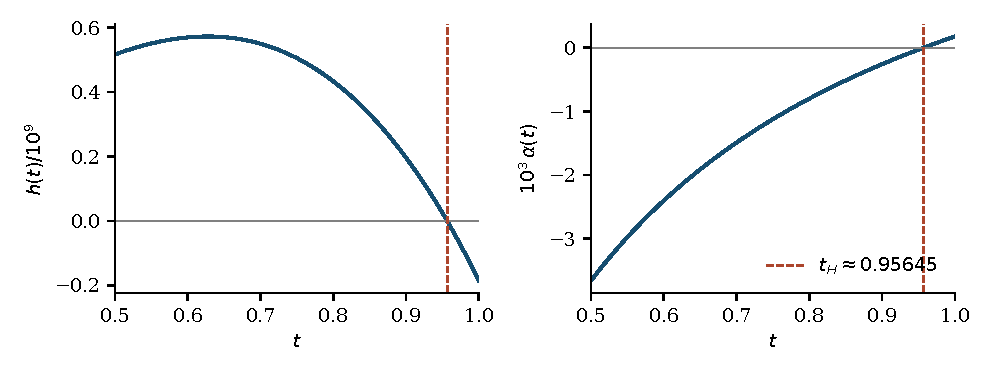
\includegraphics[width=.9\linewidth]{figures/crossing.pdf}
\caption{Left: the crossing cubic $h(t)$ of~\eqref{eq:h} on the isolating interval $[1/2,1]$. Right: the real part $\alpha(t)$ of the critical eigenvalue pair of $A(t)$. Endpoint signs, uniqueness of the zero and transversality are exact; the curves are floating-point samples and the dashed line marks the numerical value of $t_H$.}
\label{fig:crossing}
\end{figure}

\begin{remark}[Vassena's inertia-change theorem]\label{rem:vassena}
Proposition~\ref{prop:crossing} places $\Osc$ under~\cite[Theorem~5.2]{Vassena2025Hopf} (numbering of the arXiv version): $S$ has full row rank, $\vbar>0$ lies in $\ker S$, $S\diag(\vbar)Y^{\mathsf T}$ is invertible (its determinant is $48\cdot24\cdot3000$), and the concentration scalings $\diag(\xbar(t))^{-1}$ for $t<t_H$ and $t>t_H$ give matrices of different inertia. That theorem yields, by a global Hopf argument, the existence of rate constants with nonstationary periodic solutions. It is an independent conventional proof of Theorem~\ref{thm:main}(1). The next section gives the local analytic construction that is actually formalized, which also delivers the branch structure used later.
\end{remark}

\section{Periodic existence by localized shooting}\label{sec:shooting}

\subsection{Amplitude blow-up and moving eigenvectors}

Write $z=\ones+ru$ with amplitude $r\in\R$ and divide out the amplitude:
\begin{equation}\label{eq:blowup}
G(t,r,u)=\begin{cases}F_t(\ones+ru)/r,&r\ne0,\\ A(t)u,&r=0.\end{cases}
\end{equation}
Because $F_t$ is polynomial in $z$ with $F_t(\ones)=0$, the polynomial $F_t(\ones+ru)$ in $(t,r,u)$ is divisible by $r$, and $G$ is a polynomial, hence smooth, on all of $\R\times\R\times\R^4$; no singular extension is involved. If $u$ solves $\dot u=G(t,r,u)$ with $\ones+ru>0$, then $z=\ones+ru$ solves~\eqref{eq:F}.

\begin{lemma}[Explicit eigenvectors]\label{lem:eigvec}
Let $\lambda\in\C$ and $t>0$ with $\lambda\ne-1$ and $\lambda\ne-2/25$, and define
\begin{equation}\label{eq:q}
q_1=\frac{-398}{\lambda+1},\qquad
q_3=\frac{2\lambda+402t+t\,q_1}{375t},\qquad
q_2=\frac{1-q_3}{25\lambda+2},\qquad q_4=1 .
\end{equation}
Then rows $1$, $2$ and $4$ of $(A(t)-\lambda I)q=0$ hold identically, and row $3$ holds if and only if $p_t(\lambda)=0$. Consequently, for $t$ near $t_H$ the eigenvalue $\lambda(t)=\alpha(t)+i\beta(t)$ has the smooth eigenvector $q(t)=u(t)+iv(t)$ given by~\eqref{eq:q}, with $q_4\equiv1$.
\end{lemma}

\begin{proof}
Row $1$ is $-(1+\lambda)q_1-398=0$; row $4$ is $-\tfrac t2q_1+\tfrac{375t}{2}q_3-(201t+\lambda)=0$; row $2$ is $-(\tfrac{2}{25}+\lambda)q_2-\tfrac1{25}q_3+\tfrac1{25}=0$; each is solved by~\eqref{eq:q}. Substituting~\eqref{eq:q} into row $3$ and clearing denominators leaves a polynomial in $\lambda$ that is congruent to zero modulo $p_t(\lambda)$ (an exact reduction performed by \texttt{check\_paper.py}), so row $3$ holds whenever $p_t(\lambda)=0$. At $\lambda=i\omega_H$ the excluded values are avoided, and smoothness in $t$ follows from smoothness of $\lambda(t)$.
\end{proof}

At $t_H$, with $A=A(t_H)$, the real and imaginary parts satisfy $Au=-\omega_Hv$ and $Av=\omega_Hu$. Let $e,f$ be real eigenvectors of $A$ for $\lambda_s,\lambda_f$. The four vectors $u,v,e,f$ are linearly independent: the centre plane is annihilated by $A^2+\omega_H^2I$, which is invertible on the span of $e,f$ (its eigenvalues there are $\lambda_s^2+\omega_H^2$ and $\lambda_f^2+\omega_H^2$, both positive), and $e,f$ are separated by their distinct eigenvalues.

\subsection{The return defect and its derivative}

Let $T_H=2\pi/\omega_H$. For amplitude $r$ and unknowns $(t,P,a,b)$ start $\dot u=G(t,r,u)$ at
\begin{equation}\label{eq:u0}
u_0(t,a,b)=u(t)+ae+bf
\end{equation}
and let $\mathcal R(r,t,P,a,b)\in\R^4$ be the time-$P$ endpoint minus $u_0$. Then $\mathcal R(0,t_H,T_H,0,0)=0$, because at $r=0$ the equation is linear and $u(t_H)$ lies on the $T_H$-periodic centre orbit.

\begin{lemma}[A $C^1$ endpoint map on a common neighbourhood]\label{lem:cutoff}
There are a neighbourhood $\mathcal U$ of $(0,t_H,T_H,0,0)$ and a $C^1$ map $\mathcal R\colon\mathcal U\to\R^4$ with the following property: for every $(r,t,P,a,b)\in\mathcal U$ the solution of $\dot u=G(t,r,u)$ with $u(0)=u_0(t,a,b)$ exists on $[0,P]$ and $\mathcal R(r,t,P,a,b)$ is its endpoint minus $u_0$.
\end{lemma}

\begin{proof}
Append the constant coordinates $t,r,P$ and pass to unit time: the augmented field $(u,t,r,P)\mapsto(PG(t,r,u),0,0,0)$ is smooth. Multiply it by a smooth cutoff $\chi$ equal to one on a closed ball $B$ that contains the compact base orbit $\{(e^{sA}u(t_H),t_H,0,T_H):s\in[0,1]\}$ with positive margin, and zero outside a larger ball. The resulting field $g$ has compact support, bounded derivative and a global Lipschitz constant, so Picard iteration gives a global flow $\Phi$, and the variational equation with Gronwall's inequality gives continuous differentiability of $\Phi(s,\cdot)$ on short time intervals; composition extends it to time one. By continuous dependence and compactness, for all initial data in a neighbourhood $\mathcal U$ of the base point the unit-time trajectory of $g$ stays in $B$, where $g$ is the augmented field. There the $u$-component of $\Phi(1,\cdot)$ is the time-$P$ endpoint of $\dot u=G(t,r,u)$, and $\mathcal R$ is its difference with $u_0$, which is $C^1$.
\end{proof}

\begin{proposition}[The bordered derivative]\label{prop:border}
At $(0,t_H,T_H,0,0)$ the four columns of $D_{(t,P,a,b)}\mathcal R$ are
\begin{equation}\label{eq:border}
T_H\alpha'(t_H)\,u-T_H\beta'(t_H)\,v,\qquad -\omega_H\,v,\qquad (e^{\lambda_sT_H}-1)\,e,\qquad (e^{\lambda_fT_H}-1)\,f ,
\end{equation}
and they are linearly independent.
\end{proposition}

\begin{proof}
At $r=0$ the equation is $\dot u=A(t)u$, and the solution from $u(t)$ is the real part of $e^{\lambda(t)s}q(t)$:
\[
e^{\alpha(t)s}\bigl(\cos(\beta(t)s)\,u(t)-\sin(\beta(t)s)\,v(t)\bigr).
\]
At $s=T_H$ and $t=t_H$ this equals $u(t_H)$. Differentiating the endpoint minus $u(t)$ with respect to $t$ at $t_H$: the term $u'(t)$ cancels against $-u'(t)$, the term $v'(t)$ carries the factor $\sin(\omega_HT_H)=0$, and what remains is $T_H\alpha'(t_H)u-T_H\beta'(t_H)v$ (using $\cos(\omega_HT_H)=1$). Differentiating in $P$ gives the velocity $Au(t_H)=-\omega_Hv$ at the base point. The $a$ and $b$ derivatives are the linear flow applied to $e$ and $f$, minus $e$ and $f$. The vectors $u,v,e,f$ are independent, $T_H\alpha'(t_H)\ne0$ by Proposition~\ref{prop:transversal}, $\omega_H\ne0$, and $e^{\lambda T_H}\ne1$ for $\lambda\in\{\lambda_s,\lambda_f\}$ real and negative. Expressing the four columns in the basis $u,v,e,f$ gives a block-triangular coefficient matrix with nonzero diagonal, so the columns are independent.
\end{proof}

\subsection{Proof of Theorem~\ref{thm:main}}

\begin{proof}[Proof of Theorem~\ref{thm:main}]
Item~(2) is Theorem~\ref{thm:children} and item~(3) is Theorem~\ref{thm:deletion}. For item~(1), Lemma~\ref{lem:cutoff} and Proposition~\ref{prop:border} let the implicit-function theorem produce $\varepsilon>0$ and $C^1$ functions $(t(r),P(r),a(r),b(r))$ on $(-\varepsilon,\varepsilon)$, through $(t_H,T_H,0,0)$ at $r=0$, with $\mathcal R(r,t(r),P(r),a(r),b(r))=0$. Shrinking $\varepsilon$, all the returning unit-time segments lie in the ball $B$ of Lemma~\ref{lem:cutoff} (uniform localization), hence are bounded by a constant $R$ independent of $r$; for $|r|<1/R$ the physical trajectory $z=\ones+ru$ is strictly positive on the segment. At $r=0$ the initial velocity is $A(t_H)u(t_H)=-\omega_Hv(t_H)\ne0$, and continuity of $G$ and of the branch gives a nonzero initial velocity for all small $r$, so the returning solution is nonconstant. By uniqueness of solutions of the smooth ODE, the returning segment on $[0,P(r)]$ extends to a $P(r)$-periodic solution on all of $\R$ that satisfies the equation at every time, including the joins. Finally $x_i(s)=\xbar_i(t(r))\,z_i(s)$ conjugates~\eqref{eq:F} to the literal system~\eqref{eq:system} at rates $k(t(r))$, which are positive. Fix any $r\in(0,\varepsilon)$ with $r<1/R$.
\end{proof}

\begin{corollary}[The local branch]\label{cor:branch}
There are $\varepsilon>0$, functions $t(r),P(r)$ on $(0,\varepsilon)$, and positive nonconstant periodic solutions $x_r$ of~\eqref{eq:system} at rates $k(t(r))$ with period $P(r)$ such that, as $r\downarrow0$,
\[
t(r)\to t_H,\qquad P(r)\to T_H,\qquad
\sup_{0\le\theta\le1}\Bigl\|\frac{x_r(P(r)\theta)}{\xbar(t(r))}-\ones\Bigr\|\to0,
\]
the quotient being coordinatewise. The period $P(r)$ is a period, not necessarily the least period.
\end{corollary}

\begin{proof}
The implicit functions converge to their base values. Uniform continuity of the localized flow on a compact parameter neighbourhood times $[0,1]$ bounds the displacement $u$ uniformly, and multiplication by $r$ gives the displayed uniform limit. Positivity and nonzero velocity hold throughout a sufficiently small amplitude interval by the proof above.
\end{proof}

\section{Attraction and persistence: a rational certificate}\label{sec:stability}

This section is a conventional computer-assisted strengthening of Theorem~\ref{thm:main}, separate from the compiled existence theorem. Set $y=z-\ones$ and expand the field~\eqref{eq:F} at $t_H$ in unchanged time:
\[
F_{t_H}(\ones+y)=Ay+\tfrac12B(y,y)+\tfrac16C(y,y,y)+O(\|y\|^4),
\]
so that $B$ and $C$ are the second and third derivatives at $\ones$, with no factorials absorbed. For an ordered index tuple $(i_1,\dots,i_d)$ with multiplicities $\nu_i=\#\{s:i_s=i\}$, the entries are exactly
\begin{equation}\label{eq:jets}
\partial_{i_1}\cdots\partial_{i_d}F_{t_H,a}(\ones)=\xbar_a(t_H)^{-1}\sum_{j=1}^5S_{aj}\vbar_j\prod_{i=1}^4(Y_{ij})_{\nu_i},
\qquad (n)_m=n(n-1)\cdots(n-m+1),
\end{equation}
since $\partial_i^{\nu}z_i^{Y_{ij}}=(Y_{ij})_\nu$ at $z_i=1$. This is the formula evaluated by the certificate.

Let $q$ and $p$ satisfy $Aq=i\omega_Hq$, $A^{\mathsf T}p=-i\omega_Hp$ and $\langle p,q\rangle:=\bar p^{\mathsf T}q=1$. The first Lyapunov coefficient, in the invariant form of~\cite[\S5.4]{Kuznetsov2004}, is
\begin{equation}\label{eq:l1}
\ell_1=\frac{1}{2\omega_H}\Real\Bigl\langle p,\;C(q,q,\bar q)-2B\bigl(q,A^{-1}B(q,\bar q)\bigr)+B\bigl(\bar q,(2i\omega_HI-A)^{-1}B(q,q)\bigr)\Bigr\rangle .
\end{equation}
Replacing $q$ by $cq$ with $c>0$ and $p$ by $p/c$ multiplies~\eqref{eq:l1} by $c^2$; replacing $q$ by $e^{i\theta}q$ leaves it unchanged. So the sign of $\ell_1$ is well defined and its value is fixed by a normalization of $\|q\|$.

\begin{lemma}[Rational enclosure of the Lyapunov coefficient]\label{lem:interval}
With $\|q\|_2=1$, the coefficient~\eqref{eq:l1} satisfies
\[
-\frac{23}{1000}<\ell_1<-\frac{22}{1000}.
\]
Numerically $\ell_1\approx-0.0223997$.
\end{lemma}

\begin{proof}[Computer-assisted proof]
The script \texttt{amplitude\_enclosure.py} works with intervals whose endpoints are rationals on the dyadic grid $2^{-100}\Z$, rounding every real operation outward; complex numbers are pairs of such intervals, and no floating-point quantity enters any acceptance test. It proceeds as follows.

\emph{Enclosing $t_H$ and $\omega_H$.} Starting from $[1/2,1]$ it bisects $110$ times, retaining at each step the half on which $h$ has opposite signs at the endpoints (exact rational evaluation). By Proposition~\ref{prop:crossing} the exact $t_H$ lies in the final interval. It encloses $\omega_H^2=a_3/a_1$ by interval arithmetic and $\omega_H$ by a rational bracket $[w_l,w_h]$ with $w_l^2\le\underline{\omega^2}$ and $w_h^2\ge\overline{\omega^2}$, again exact inequalities.

\emph{Enclosing the eigenvectors.} Let $M=A-i\omega_HI$ with $A$ evaluated on the $t$-interval. Interval Gaussian elimination with recorded pivots solves the first three equations of $Mq=0$ with $q_4=1$, and the first three equations of $\ell M=0$ for a row vector $\ell$ with $\ell_4=1$. Each pivot is accepted only if the lower endpoint of its squared modulus interval is strictly positive; the $14$ pivots used are stored in the certificate. Hence the leading $3\times3$ block of $M$ is invertible for the exact enclosed objects. Since $\det M=p_{t_H}(i\omega_H)=0$ by~\eqref{eq:factor}, the scalar Schur complement of that block is zero, so the omitted fourth equations hold exactly for both vectors: $q$ is a right eigenvector and $\ell$ a left eigenvector of $A$ for $i\omega_H$. The interval for the pairing $\ell q$ excludes zero; replacing $\ell$ by $\ell/(\ell q)$ gives exactly $\ell=\bar p^{\mathsf T}$ in the convention of~\eqref{eq:l1}, because $A^{\mathsf T}p=-i\omega_Hp$ is equivalent to $\bar p^{\mathsf T}A=i\omega_H\bar p^{\mathsf T}$.

\emph{Resolvents and contraction.} The same checked elimination encloses $A^{-1}B(q,\bar q)$ and $(2i\omega_HI-A)^{-1}B(q,q)$; both matrices are invertible for the exact objects since $0$ and $2i\omega_H$ are not eigenvalues of $A$ by~\eqref{eq:factor}. The jets~\eqref{eq:jets} are exact rationals, and the contractions of~\eqref{eq:l1} are evaluated in interval arithmetic. Inclusion is inductive: every interval operation contains the corresponding exact operation, and every division has a denominator interval excluding zero. Dependency overestimation can only widen the result.

\emph{Result.} With $q_4=1$ the enclosure of $\ell_1$ is a negative interval of width below $10^{-16}$ centred near $-3512.397595509238$, and the enclosure of $\|q\|_2^2$ is a positive interval centred near $156805.5821151$. Dividing, and using the scaling law noted after~\eqref{eq:l1} with $c=\|q\|_2^{-1}$, gives an interval for the unit-norm coefficient centred near $-0.02239969743507$ whose endpoints satisfy the two displayed rational inequalities. The rational endpoints, not the printed centres, are the acceptance test; they are stored in \texttt{amplitude\_enclosure.json} together with all pivots.
\end{proof}

A floating-point evaluation of~\eqref{eq:l1} (in \texttt{check\_paper.py}) reproduces the centre to twelve digits; it is used for orientation only.

\begin{proof}[Proof of Theorem~\ref{thm:attract}]
At $t_H$ the field~\eqref{eq:F} is smooth, its equilibrium $\ones$ has the simple purely imaginary pair $\pm i\omega_H$ with $\omega_H>0$, the remaining eigenvalues $\lambda_s,\lambda_f$ are real and negative (Lemma~\ref{lem:factor}), the pair crosses the axis with $\alpha'(t_H)>0$ (Proposition~\ref{prop:transversal}), and $\ell_1<0$ (Lemma~\ref{lem:interval}). These are the hypotheses of the nondegenerate Hopf theorem in $\R^n$ (centre-manifold reduction followed by the planar theorem, \cite[\S\S3.4--3.5 and \S5.4]{Kuznetsov2004}). In the reduced normal form $\dot\rho=\rho(\alpha(t)+\ell_1\rho^2+\dots)$, the radius $\rho\approx\sqrt{-\alpha(t)/\ell_1}$ is positive exactly for $t>t_H$, and the derivative of the radial field at that radius is negative; the complementary directions are contracting. Hence for $t>t_H$ close to $t_H$ there is a unique small periodic orbit, it is orbitally asymptotically stable and hyperbolic (one trivial multiplier $1$ and three multipliers of modulus below one), and it is positive because it converges to the positive equilibrium $\ones$. Undoing the normalization $x_i=\xbar_i(t)z_i$ gives the first statement.

Fix one such $t$ and consider the system~\eqref{eq:system} as a smooth function of the five rate constants near $k(t)$. On a three-dimensional transverse section the return map has the periodic orbit as a fixed point with three multipliers strictly inside the unit circle, so the derivative of the return map minus the identity is invertible. The return map depends smoothly on the rates, and the implicit-function theorem continues the fixed point to a neighbourhood $\mathcal K$ of $k(t)$ in $\R^5$, which can be taken inside $\R_{>0}^5$. Multipliers vary continuously, so the continued orbit remains hyperbolic and attracting on a possibly smaller neighbourhood; compactness of the orbit and continuity keep it in the positive orthant. Theorems~\ref{thm:children} and~\ref{thm:deletion} depend only on the source, so they continue to hold at every point of $\mathcal K$.
\end{proof}

Theorem~\ref{thm:attract} does not certify any explicit endpoint of the open region, and does not validate a periodic orbit at any specific decimal rate vector. Its proof is complete as a conventional argument with the rational certificate; neither the Lyapunov coefficient nor the Hopf stability theorem is compiled in Lean.

\section{Exact averages and the oscillatory concentration shift}\label{sec:means}

\begin{proposition}[Period averages]\label{prop:means}
Let $x$ be a positive $P$-periodic solution of~\eqref{eq:system} at rates $k\in\R_{>0}^5$, and write $\av f=P^{-1}\int_0^Pf(x(s))\,ds$. Then
\begin{equation}\label{eq:means}
\av{v}=(k_5,\tfrac32k_5,k_5,k_5,k_5),
\end{equation}
which is the equilibrium flux at the same rates. With $z_i=x_i/x_i^*$ for the equilibrium $\xs$ of Proposition~\ref{prop:eq},
\begin{equation}\label{eq:moments}
\av{z_1z_4^{400}}=\av{z_2^4z_3^2}=\av{z_3^{375}}=\av{z_4^2}=1 .
\end{equation}
In particular $\av{z_4}^2+\Var(z_4)=1$ and $\av{z_3}\le1$.
\end{proposition}

\begin{proof}
Integrating~\eqref{eq:ode} over a period gives $S\int_0^Pv(x(s))\,ds=x(P)-x(0)=0$, so $\int_0^Pv\,ds\in\ker S$ is a multiple of $(2,3,2,2,2)$, and its fifth entry is $Pk_5$; this is the compiled identity \lean{periodic_integrated_flux}. Dividing by $P$ gives~\eqref{eq:means}. Each equilibrium flux equals the same rate constant times the equilibrium monomial, so dividing each entry of~\eqref{eq:means} by $v_j(\xs)$ gives~\eqref{eq:moments}. The variance identity is $\av{z_4^2}=\av{z_4}^2+\Var(z_4)$, and $\av{z_3}\le\av{z_3^{375}}^{1/375}=1$ by Jensen's inequality for the convex function $y\mapsto y^{375}$ on $\R_{>0}$.
\end{proof}

\begin{proposition}[Strict mean shift]\label{prop:shift}
Every nonconstant positive periodic solution of~\eqref{eq:system} at positive rates satisfies $\av{x_4}<x_4^*$.
\end{proposition}

\begin{proof}
Suppose $x_4$ were constant, $x_4\equiv c>0$. Then $\dot x_1=-k_1c^{400}x_1+k_4c^2$ is a scalar linear equation whose only periodic solution is its constant equilibrium (a nonconstant solution is a nonzero exponential plus a constant, which is not periodic). Hence $x_1$ is constant. The fourth equation of~\eqref{eq:system} with $\dot x_4=0$ and $x_1,x_4$ constant forces $k_3x_3^{375}$ constant, hence $x_3$ constant; the third equation then forces $k_2x_2^4x_3^2$ constant, hence $x_2$ constant. The solution would be constant. Therefore $z_4$ is a nonconstant continuous periodic function and $\Var(z_4)>0$, so $\av{z_4}^2<1$ by~\eqref{eq:moments}, and $\av{z_4}<1$ since $\av{z_4}>0$.
\end{proof}

No average of a product in~\eqref{eq:moments} has been factored into a product of averages, and Proposition~\ref{prop:shift} does not use attraction: it holds for every positive periodic solution.

\section{Numerical illustration and scope}\label{sec:numerics}

\subsection{A shooting illustration}

Figure~\ref{fig:orbit} shows the local branch of Corollary~\ref{cor:branch} in relative concentrations at amplitude $r=0.02$, computed by the implicit midpoint method applied to the blown-up equation~\eqref{eq:blowup}. The initial displacement is fixed in a numerical real eigenbasis at the crossing ($u_0=u+ae+bf$ as in~\eqref{eq:u0}), and the two stable coordinates $a,b$, the parameter $t$ and the period $P$ are solved from the four return equations by Newton's method with finite-difference derivatives. Each midpoint Newton solve stops at correction norm below $2\cdot10^{-13}$ and the shooting residual tolerance is $2\cdot10^{-9}$. Since $\lambda_f\approx-195$, explicit long-step integration is inappropriate, which motivates the implicit method.

\begin{table}[ht]
\centering
\begin{tabular}{rrr}
\toprule
Midpoint steps & Parameter $t$ & Returned period $P$\\
\midrule
128 & 0.956506609271 & 62.2226143528\\
256 & 0.956506654719 & 62.2132421634\\
512 & 0.956506666084 & 62.2108996453\\
\bottomrule
\end{tabular}
\caption{Discrete shooting at amplitude $r=0.02$. Refinement changes the period at the second-order scale expected of the midpoint rule; $t-t_H\approx5.3\cdot10^{-5}>0$ is consistent with the supercritical direction of Theorem~\ref{thm:attract}. These are floating-point values from a discrete scheme, not validated properties of a continuous-time orbit.}
\label{tab:shooting}
\end{table}

\begin{figure}[ht]
\centering
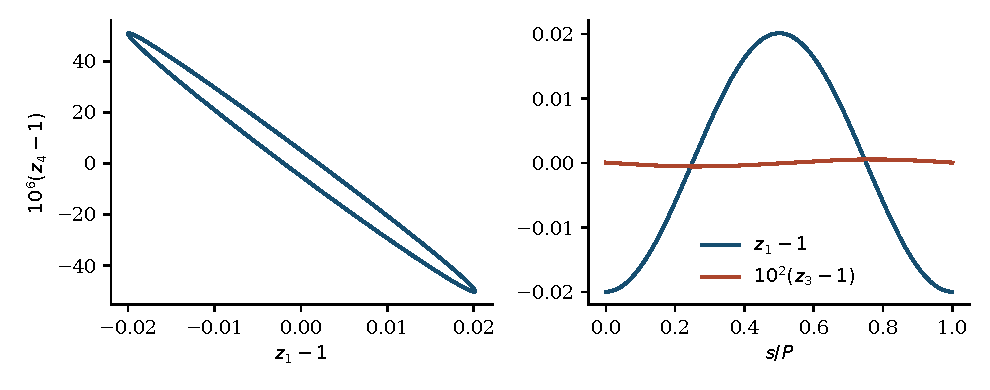
\includegraphics[width=\linewidth]{figures/orbit.pdf}
\caption{The shooting illustration at $512$ midpoint steps: a projection of the relative-concentration orbit onto $(z_1,z_4)$ (the vertical scale makes the small fourth-coordinate variation visible), and the time traces of $z_1-1$ and $z_3-1$ over one period. This is neither a validated continuous-time orbit at the printed parameter nor a numerical proof of stability.}
\label{fig:orbit}
\end{figure}

At $512$ steps the midpoint-quadrature means of the five flux ratios $v_j/v_j(\xs)$ differ from one by at most $1.4\cdot10^{-15}$, and the mean of $z_4$ is $0.99999999936<1$; these agree with~\eqref{eq:moments} and Proposition~\ref{prop:shift} to the accuracy of the scheme and serve as implementation checks, not as independent certificates.

\subsection{Interpretation and what is not claimed}

The result isolates a collective effect. No individual child-selection matrix of $\Osc$ can be destabilized by diagonal scaling, yet the full reactivity, which weights the same stoichiometric columns by kinetic orders and equilibrium concentrations, produces a Hopf bifurcation and an attracting periodic orbit. The kinetic orders are decisive: by~\cite[Theorem~5.2]{KineticOrder2026}, the skeleton $(Y_0,P_0)$ of Lemma~\ref{lem:padding} is Hurwitz stable at every positive mass-action equilibrium, so the padding entries $371$ and $398$ are responsible for everything dynamical here. Every positive rate vector gives a unique nonsingular equilibrium, and an open set of rate vectors supports attracting periodic motion around it.

We do not claim: global attraction of the periodic orbit or of the equilibrium for any rates; minimality of the kinetic orders $400$ and $375$ on this skeleton (see~\cite[Question~8.2]{KineticOrder2026}, where order $200$ suffices for linear instability); minimality of the network among all mass-action oscillators, which fails since bimolecular Hopf networks with three species exist~\cite{BanajiBoros2023}; a low-molecularity, thermodynamically closed, or laboratory realization. $\Osc$ is an open classical mass-action model, with inflow $r_5$ and outflow $r_2$, whose deletion minimality is relative to its own five reactions.

\section{Formal verification and reproducibility}\label{sec:formal}

\subsection{The compiled statements}

Theorem~\ref{thm:main}(1), (2) and the periodic part of~(3) are verified in Lean~4~\cite{Lean4} with Mathlib~\cite{Mathlib}, compiled with warnings treated as errors and no unproved placeholders, against the frozen toolchain \lean{leanprover/lean4:v4.30.0}. The development lives in \lean{proofs/OscillatoryCores/} of the accompanying repository and imports the source-network, child-selection, $D$-scaling and mass-action interfaces of the companion developments~\cite{ParameterRich2026,KineticOrder2026}. The source is the literal \lean{SourceNetwork} \lean{source} with the reactant and product matrices~\eqref{eq:matrices}; \lean{State} is $\R^4$; \lean{Solves k x} states that every coordinate of $x\colon\R\to\R^4$ has, at every time, derivative equal to the corresponding right side of~\eqref{eq:system} with rates $k$; \lean{ChildSelection source} is Definition~\ref{def:child} with reactant incidence $Y_{ij}>0$; \lean{DNonUnstable} is $D$-nonunstability under diagonal scaling; and \lean{IsDUnstableCore} is a $D$-unstable child selection minimal under restriction. The two public declarations are, in ASCII rendering,
\begin{verbatim}
theorem literal_oscillator_resolution :
  (exists k : Fin 5 -> R, exists x : R -> State, exists P : R,
     (forall j, 0 < k j) and 0 < P and (forall s i, 0 < x s i) and
     Solves k x and Function.Periodic x P and (exists s, x s /= x 0)) and
  (forall kappa : ChildSelection source, DNonUnstable kappa.realMatrix) and
  (forall k : Fin 5 -> R, (forall j, 0 <= k j) ->
     forall j0 : Fin 5, k j0 = 0 ->
     forall x : R -> State, (forall s i, 0 < x s i) -> Solves k x ->
     forall P : R, 0 < P -> Function.Periodic x P -> forall s, x s = x 0)

theorem literal_no_dUnstableCore :
  not (exists kappa : ChildSelection source, IsDUnstableCore kappa)
\end{verbatim}
in the namespace \lean{OscillatoryCores}. The first conjunct is item~(1) with an all-real-time positive nonconstant periodic solution of the literal ODE; the second is item~(2); the third is the periodic sentence of item~(3) at arbitrary nonnegative retained rates.

Two further compiled declarations support Sections~\ref{sec:flux} and~\ref{sec:means}: \lean{deletion_observable_hasDerivAt} in \lean{PublicationConsequences.lean} is the identity~\eqref{eq:observable} for every solution of the deleted system, with the covectors~\eqref{eq:weights} as literal data, and \lean{periodic_integrated_flux} in the same file identifies the period integral of the flux vector of any returning solution with $Pk_5\cdot(1,\tfrac32,1,1,1)$, which is~\eqref{eq:means} before division by $P$. The declaration \lean{local_return_family} in \lean{LocalBranchCorollaries.lean} exports the local returning family of Section~\ref{sec:shooting}: a continuous family of initial states and parameters and, for every sufficiently small amplitude, positive parameter and period, uniform localization and positivity of the unit-time segment, exact return, and nonzero displacement velocity. It retains the base parameter and period but does not identify them in its interface with the displayed spectral constants $t_H$ and $T_H$; that identification and the uniform-limit statement of Corollary~\ref{cor:branch} are conventional.

\subsection{Module map and receipts}

Table~\ref{tab:lean} maps the mathematical steps to Lean modules. The child-safety module transports, through the reactant-incidence identity of Lemma~\ref{lem:padding}, a kernel-checked replay of the child certificates of~\cite[Theorem~4.7]{ParameterRich2026}; the finite decision procedures of the original development were replaced by kernel-reduced proofs, so no native-computation axiom enters. The verification receipts record exit code zero, no compiler output, and axiom reports containing only \lean{propext}, \lean{Classical.choice} and \lean{Quot.sound}; no \lean{sorryAx} appears. The root receipt covers $94$ dependency sources. The SHA-256 of the root source \lean{Resolution.lean} and of the frozen Lake manifest are
\begin{center}\small
\lean{e646d6406d4dbfb7d365260d8b01b4ba75a1ecb4cbd285d1bdcd92879fcc38cd}\\
\lean{a8df0b606ec258561c226df89856884be433c19b49fb0a27335d69bb2b6e9fac}
\end{center}

\begin{table}[ht]
\centering\footnotesize
\begin{tabular}{@{}>{\raggedright\arraybackslash}p{0.34\linewidth}>{\raggedright\arraybackslash}p{0.60\linewidth}@{}}
\toprule
Mathematical step & Modules under \lean{proofs/OscillatoryCores/}\\
\midrule
Literal source, flux circuit, rate reconstruction (Section~\ref{sec:source}, Lemma~\ref{lem:circuit}) & \lean{Source.lean}, \lean{FluxCircuit.lean}\\
\addlinespace
Child exclusion (Theorem~\ref{thm:children}) & \lean{KernelChildCertificate.lean}, \lean{ChildTransport.lean}, \lean{ChildSafety.lean}\\
\addlinespace
Integrated ODE and deletion (Theorem~\ref{thm:deletion}, periodic part) & \lean{PeriodicMeanFlux.lean}, \lean{DeletionMinimality.lean}\\
\addlinespace
Exact spectrum and moving eigenvectors (Section~\ref{sec:crossing}, Lemma~\ref{lem:eigvec}) & \lean{Jacobian.lean}, \lean{QuarticCertificates.lean}, \lean{SpectrumCertificate.lean}, \lean{SpectralCrossing.lean}, \lean{SpectralTransversality.lean}, \lean{EigenvectorFormula.lean}, \lean{MovingBranch.lean}\\
\addlinespace
Cutoff flow and shooting (Lemma~\ref{lem:cutoff}, Proposition~\ref{prop:border}) & \lean{CutoffFlow.lean}, \lean{FlowRegularity.lean}, \lean{ShootingDerivative.lean}, \lean{ShootingBranch.lean}, \lean{LiteralShootingBranch.lean}\\
\addlinespace
Positive periodic transport (proof of Theorem~\ref{thm:main}(1)) & \lean{NonzeroShootingPoint.lean}, \lean{AmplitudeOrbit.lean}, \lean{PeriodicOrbit.lean}\\
\addlinespace
Root theorem & \lean{Resolution.lean}\\
\addlinespace
Deletion covectors and period integrals (Proposition~\ref{prop:covectors}, \eqref{eq:means}) & \lean{PublicationConsequences.lean}\\
\addlinespace
Local returning family & \lean{LocalBranchCorollaries.lean}\\
\bottomrule
\end{tabular}
\caption{Mathematical steps and the Lean modules that verify them.}
\label{tab:lean}
\end{table}

\subsection{Conventional statements}

The following are proved in this paper by ordinary mathematics and are not separately formalized: the existence and uniqueness of the positive equilibrium for all positive rates and the determinant formula (Proposition~\ref{prop:eq}); the equilibrium, return and recurrence sentences of Theorem~\ref{thm:deletion} beyond the compiled derivative identity, and Remark~\ref{rem:circuit}; the Routh--Hurwitz inertia count in Proposition~\ref{prop:crossing} (the Lean development proves the exact factorization~\eqref{eq:factor}, the unique root, and transversality on its own route); Corollary~\ref{cor:branch} in its displayed form; Lemma~\ref{lem:interval} (an exact rational computation, but not a Lean proof) and Theorem~\ref{thm:attract}, including the Hopf theorem and the return-map continuation; Propositions~\ref{prop:means} and~\ref{prop:shift} beyond the compiled integrated-flux identity. Remark~\ref{rem:vassena} quotes a published theorem that is not an imported dependency of the Lean proof. The numerical values in Section~\ref{sec:numerics} and the figures are illustrations, not evidence for any statement.

\subsection{Reproducibility}

The package accompanying this paper contains \texttt{check\_paper.py}, which re-derives in exact rational arithmetic (SymPy and \texttt{fractions}) every constant printed above: the matrices and the padding relation, the kernel and the minors, the equilibrium and its determinant, the twenty covector identities, the $24$ children and the six certificates with all principal minors, the normalized Jacobian~\eqref{eq:A}, the coefficients~\eqref{eq:charpoly}, the identities~\eqref{eq:h}, \eqref{eq:factorid} and the crossing-direction formula, the endpoint values of $h$, the eigenvector formula~\eqref{eq:q} modulo $p_t$, and the coefficient bounds of Lemma~\ref{lem:factor}; it then bisects $t_H$, evaluates $\omega_H$, $T_H$, $\alpha'(t_H)$ and a floating-point $\ell_1$ for orientation, and checks the rational certificate file and the shooting table. \texttt{make\_figures.py} regenerates both figures. \texttt{amplitude\_enclosure.py} in the research workspace regenerates the rational certificate and its JSON record. From the repository root, the Lean receipts are regenerated by
\begin{verbatim}
python scripts/verify_proof.py proofs/OscillatoryCores/Resolution.lean
   --timeout 180
   --declaration OscillatoryCores.literal_oscillator_resolution
   --declaration OscillatoryCores.literal_no_dUnstableCore
\end{verbatim}
(one command; join the lines), and likewise for \lean{PublicationConsequences.lean} and \lean{LocalBranchCorollaries.lean} with their declarations. The bridge runs Lean from the frozen \lean{mathlib4_project/} directory with warnings as errors; dependencies must not be updated.

\section{Open problems}\label{sec:open}

\begin{question}[Bounded molecularity]
Is there a classical mass-action network with no $D$-unstable core, every reaction consuming at most two molecules, that admits a nonconstant positive periodic solution? The companion~\cite{ReactantBimolecular2026} gives such a network with an unstable equilibrium; whether the instability there is born in a Hopf bifurcation is open.
\end{question}

\begin{question}[Minimal kinetic order for oscillation on the skeleton]
For the skeleton $(Y_0,P_0)$ of Lemma~\ref{lem:padding}, what is the smallest maximal entry of a reactant matrix $Y$ with $\supp Y=\supp Y_0$ for which the mass-action system has a nonconstant positive periodic solution? The present paper gives the upper bound $400$; \cite[Question~8.2]{KineticOrder2026} asks the same for linear instability, with upper bound $200$.
\end{question}

\begin{question}[Global dynamics]
For rates in the open set of Theorem~\ref{thm:attract}, is the attracting periodic orbit the unique nonconstant periodic solution, and is every positive trajectory bounded and attracted either to it or to the equilibrium? Proposition~\ref{prop:shift} constrains every periodic solution but says nothing about basins.
\end{question}

\begin{question}[Formal stability]
Formalize the first Lyapunov coefficient and the nondegenerate Hopf theorem so that Lemma~\ref{lem:interval} and Theorem~\ref{thm:attract} become compiled statements. The rational certificate is already exact; what is missing is a verified centre-manifold and normal-form reduction.
\end{question}

\begin{question}[Structural localization of oscillation]
Which finite structural data beyond the child lattice, for instance flux-weighted Schur reductions or bounds on kinetic orders, suffice to localize Hopf bifurcations of mass-action networks? Any proposed criterion must reject $\Osc$ and its skeleton simultaneously, since they share all child selections but differ in every dynamical respect.
\end{question}

\bibliographystyle{plain}
\bibliography{refs}

\end{document}
